\section{Overview}
\label{sec:sepcomp:overview}

We begin by explaining our Level A and Level B notions of compositional correctness and our
techniques for establishing them (\S\ref{sec:overview:LevelA} and \S\ref{sec:overview:LevelB}).  We
also briefly give some intuition as to why it is easy to adapt CompCert's verification to employ our
new techniques, but we leave a more thorough explanation of this adaptation to subsequent sections.
Throughout the section, we keep the presentation semi-formal, abstracting away unnecessary detail to
get across the main ideas.
%   We focus on correctness of compilation
% from C to assembly, but this is merely for concreteness: the ideas
% are more general

\subsection{Compositional Correctness Level A}
\label{sec:overview:LevelA}

\begin{figure}[!t]
\begin{center}
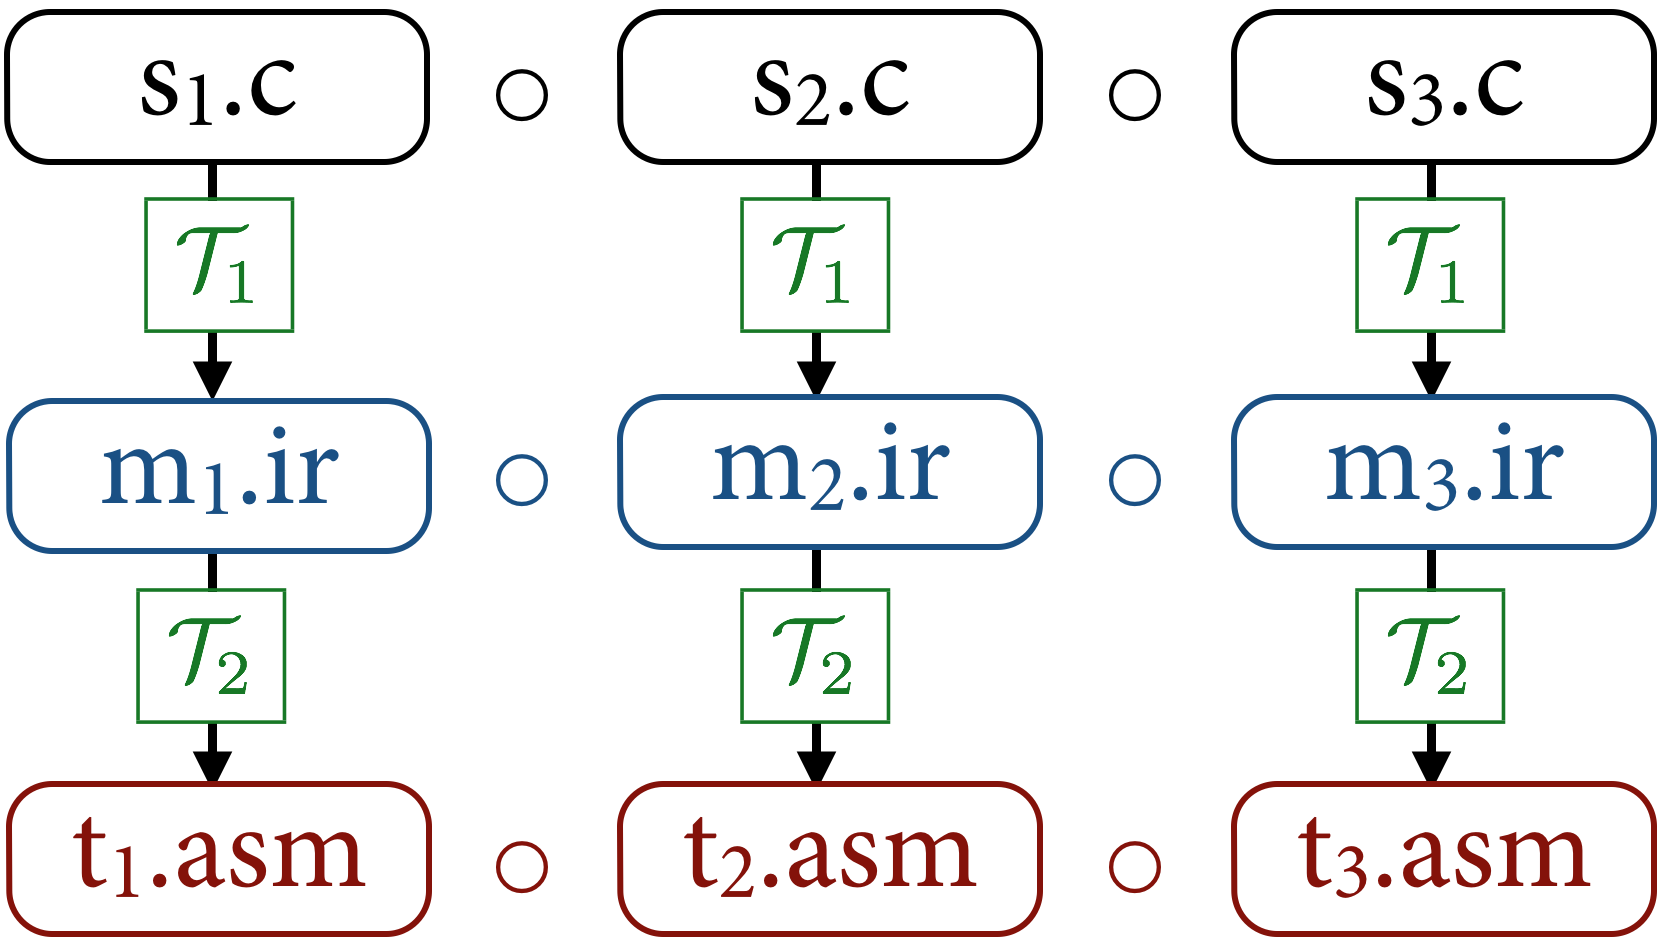
\includegraphics[width=200px]{sepcomp-levela.png}
\end{center}
\caption{Proving Level A correctness}
\label{fig:LevelA}
\end{figure}


\paragraph{End-to-End Correctness}

For Level A, we aim to show that if we separately compile $n$
different C modules
($\mathtt{s}_1\mathtt{.c},\ldots,\mathtt{s}_n\mathtt{.c}$) using the
same exact verified compiler $\mathcal{C}$, producing $n$ assembly
modules
($\mathtt{t}_1\mathtt{.asm},\ldots,\mathtt{t}_n\mathtt{.asm}$), then
the assembly-level linking of the $\mathtt{t}_i$'s will refine the
C-level linking of the $\mathtt{s}_i$'s.  Formally:
\[
\frac{
\begin{array}{@{}c@{}}
\forall i\in\setofz{1\ldots n}.~\mathcal{C}(\mathtt{s}_i\mathtt{.c}) = \mathtt{t}_i\mathtt{.asm} \\
s = \mathrm{load}(\mathtt{s}_1\mathtt{.c}\circ \ldots \circ \mathtt{s}_n\mathtt{.c})\qquad
t = \mathrm{load}(\mathtt{t}_1\mathtt{.asm}\circ \ldots \circ \mathtt{t}_n\mathtt{.asm})
\end{array}
}
{\mathrm{Behav}(s) \supseteq \mathrm{Behav}(t)}
\]
Here, $\circ$ represents simple \emph{syntactic} linking, \ie
essentially concatenation of files (plus checks to make sure that
externally declared variables/functions have the expected types).  See
\S\ref{sec:adaptconstprop} for further details about syntactic
linking.
% \footnote{See \S\ref{??} for further details about syntactic
%   linking.  Such a trivial notion of linking is no longer possible in
%   the recently released CompCert 2.5, due to the introduction of
%   support for \cd{static} variables.  See \S\ref{sec:related} for
%   further discussion of this point.}

\newcommand{\mys}[1]{\mathtt{s}_{#1}}
\newcommand{\myt}[1]{\mathtt{t}_{#1}}

\paragraph{Per-Pass Correctness}

To prove that compiler $\mathcal{C}$ satisfies Level A compositional correctness, we again want to
reduce the problem to one of verifying the individual passes of $\mathcal{C}$.  The key idea here,
as illustrated in Figure~\ref{fig:LevelA} where three separately-compiled modules go through two
compiler passes $\mathcal{T}_1$ and $\mathcal{T}_2$, is that since we know that the source modules
are all compiled via the exact same sequence of passes, we can verify their compilations in lock
step as if each pass is applied to all modules simultaneously.  In other words, it suffices to
verify that, for each pass $\mathcal{T}$ from $L_1$ to $L_2$, the following holds:
% Here, we show the case of three separately-compiled modules and two compiler passes,
% $\mathcal{T}_1$ and $\mathcal{T}_2$.  Since the compilations march in lock step, we can verify
% each pass as applied to all modules simultaneously.
\[
\frac{
\begin{array}{@{}c@{}}
\forall i\in\setofz{1\ldots n}.~\mathcal{T}(\mathtt{s}_i\mathtt{.l1}) = \mathtt{t}_i\mathtt{.l2} \\
s = \mathrm{load}(\mathtt{s}_1\mathtt{.l1}\circ \ldots \circ \mathtt{s}_n\mathtt{.l1})\qquad
t = \mathrm{load}(\mathtt{t}_1\mathtt{.l2}\circ \ldots \circ \mathtt{t}_n\mathtt{.l2})
\end{array}
}
{
\mathrm{Behav}(s) 
\supseteq \mathrm{Behav}(t)
}
\]
As before, these per-pass correctness results can be transitively
composed to immediately conclude end-to-end correctness of
$\mathcal{C}$.

\paragraph{Verifying Per-Pass Correctness}
So how do we prove this Level A per-pass correctness condition?
Assuming that we have already proven whole-program per-pass correctness
and are trying to port the proof over, there are two cases.

\textbf{Trivial case:} Many compiler passes are inherently
compositional, transforming the code of each module independently, \ie
in a way that is agnostic to the presence of other modules.  Put
another way, such compiler passes commute with linking:
\[
\mathcal{T}(\mathtt{s}_1\mathtt{.l1})\circ \ldots \circ \mathcal{T}(\mathtt{s}_n\mathtt{.l1}) = \mathcal{T}(\mathtt{s}_1\mathtt{.l1}\circ \ldots \circ \mathtt{s}_n\mathtt{.l1})
\]
If this commutativity property holds for a pass $\mathcal{T}$, then
Level A per-pass correctness becomes a trivial corollary of
whole-program per-pass correctness, where we instantiate the \cd{s.l1}
from \S\ref{sec:overview:compcert} with $\mathtt{s}_1\mathtt{.l1}\circ
\ldots \circ \mathtt{s}_n\mathtt{.l1}$.  In verifying Level A
correctness for CompCert 2.4, we found that 13 of its 19 passes fell
into this trivial case.

\textbf{Non-trivial case:} If the trivial commutativity argument does
not apply, then there is some new work to do to port a proof of
whole-program per-pass correctness to Level A per-pass correctness.

However, at least for CompCert, we found it very easy to perform this
adaptation.  Why?  First of all, since Level A correctness assumes
that all modules in the program are transformed in the same way, we
can essentially reuse the simulation relation $R$ for pass
$\mathcal{T}$ that was used in the original CompCert verification.

We do, however, have to worry about the soundness of the program
analyses that the compiler performs, because the correctness of the
compiler rests to a large extent on the correctness of these analyses.
To prove Level A correctness of these analyses, we must prove that
they remain sound even when they only have access to a single module
in the program rather than the whole program.  Intuitively, this
should follow easily if: (1) the analyses have been proven sound under
the assumption that they are fed the whole program (CompCert has done
that already), \emph{and} (2) the analyses are \emph{monotone},
meaning that they only become \emph{more conservative} when given
access to a smaller fragment of the program (as happens with separate
compilation).

In adapting CompCert to Level A correctness, the main work was
therefore in verifying that its program analyses were indeed monotone.
This was largely straightforward, with one exception: the ``value
analysis'' employed by several optimizations was not monotone.  It
made an assumption about variables declared as \cd{extern const},
which was valid for whole-program compilation, but not in the presence
of separate compilation.  As we explain in detail in
\S\ref{sec:adaptconstprop}, this manifested itself as a bug in
constant propagation when linking separately-compiled files.  After we
fixed this bug in value analysis, monotonicity became straightforward
to show, and thus so did Level A correctness (for the remaining 6
passes that did not fall into the trivial case).








% Or not:

% \[
% \frac{
% \begin{array}{@{}c@{}}
% \mathcal{T}(\mathtt{s}_1\mathtt{.l1})\circ \ldots \circ \mathcal{T}(\mathtt{s}_n\mathtt{.l1}) = \mathcal{T}(\mathtt{s}_1\mathtt{.l1}\circ \ldots \circ \mathtt{s}_n\mathtt{.l1})\\
% \mathtt{s.l1} = \mathtt{s}_1\mathtt{.l1}\circ \ldots \circ \mathtt{s}_n\mathtt{.l1}
% \\
% \mathtt{t.l2} = \mathcal{T}(\mathtt{s.l1})\qquad
% s = \mathrm{load}(\mathtt{s.l1})\qquad
% t = \mathrm{load}(\mathtt{t.l2})
% \end{array}
% }
% {
% \mathrm{Behav}(s) 
% \supseteq \mathrm{Behav}(t)
% }
% \]


\subsection{Compositional Correctness Level B}
\label{sec:overview:LevelB}

\begin{figure}[!t]
\begin{center}
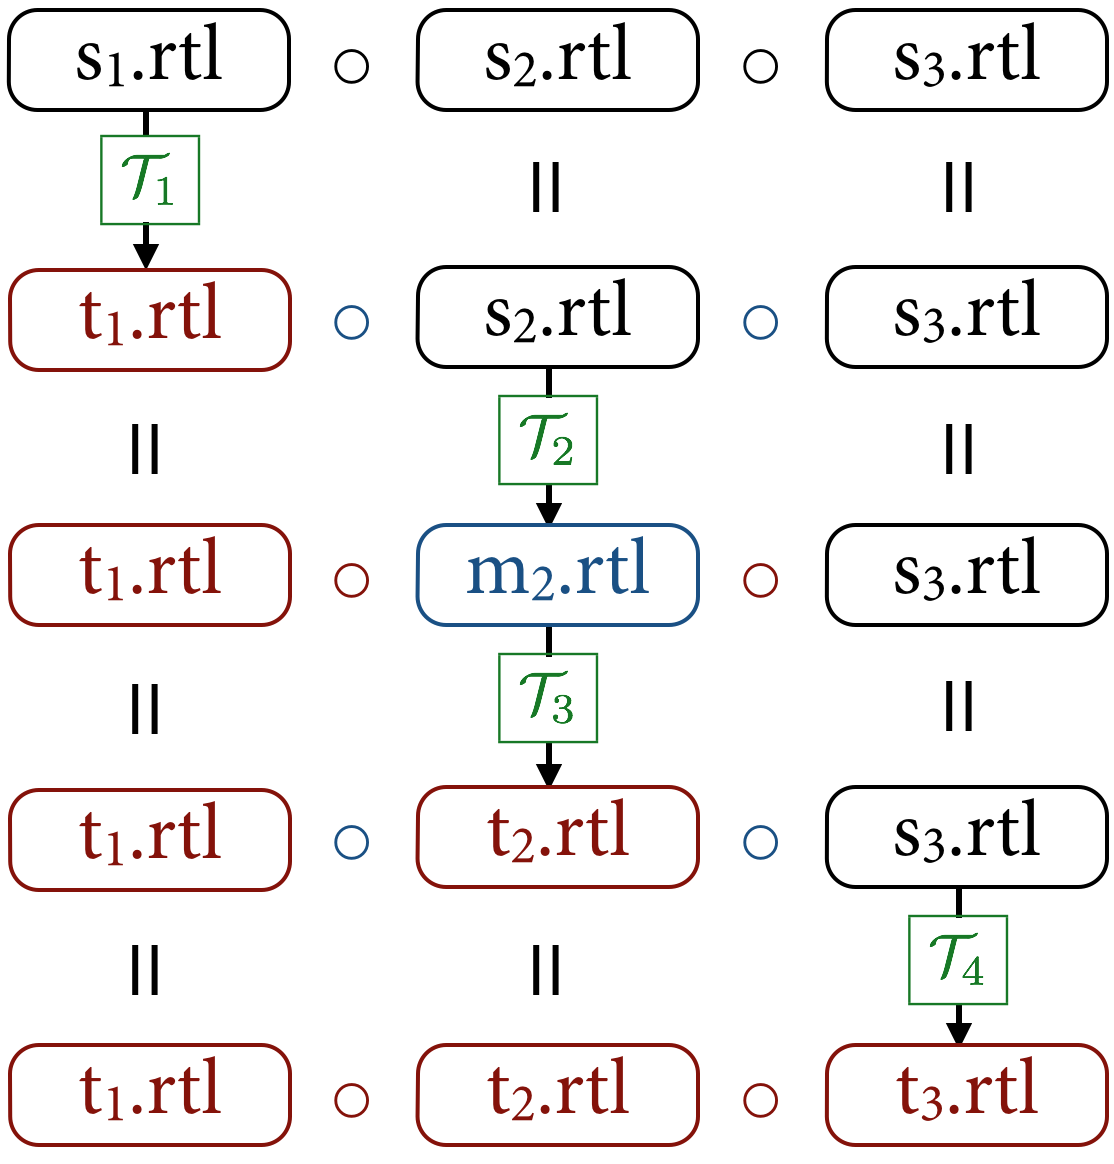
\includegraphics[width=200px]{sepcomp-levelb.png}
\end{center}
\caption{Proving Level B correctness for RTL passes}
\label{fig:LevelB}
\end{figure}
% Here, we show only the RTL-level passes (for other passes, it is the same as Level A).  Since each
% module is compiled with different optimization passes, we verify each pass applied to exactly one
% module, while simultaneously the other modules undergo the identity transformation.

\paragraph{End-to-End Correctness}

The CompCert compiler performs several key optimizations at the level
of its RTL intermediate language (\ie they are transformations from
RTL to RTL).  For Level B, we would like to strengthen Level A
correctness by allowing each source module $\mys{i}$ to be compiled by
a \emph{different} compiler $\mathcal{C}_i$.  However, the differences
we permit between the $\mathcal{C}_i$'s are restricted: they may
differ only in which optimization passes they apply at the RTL level.
Given this restriction on the $\mathcal{C}_i$'s, the Level B
correctness statement is the same as the Level A correctness statement
except for the replacement of $\mathcal{C}$ with $\mathcal{C}_i$:
\[
\frac{
\begin{array}{@{}c@{}}
\forall i\in\setofz{1\ldots n}.~\mathcal{C}_i(\mathtt{s}_i\mathtt{.c}) = \mathtt{t}_i\mathtt{.asm} \\
s = \mathrm{load}(\mathtt{s}_1\mathtt{.c}\circ \ldots \circ \mathtt{s}_n\mathtt{.c})\qquad
t = \mathrm{load}(\mathtt{t}_1\mathtt{.asm}\circ \ldots \circ \mathtt{t}_n\mathtt{.asm})
\end{array}
}
{
\mathrm{Behav}(s) 
\supseteq \mathrm{Behav}(t)
}
\]

\paragraph{Per-Pass Correctness}

To verify the above correctness statement, we yet again want to reduce
it to verifying the individual passes of $\mathcal{C}$.  For all passes
besides the RTL-level optimizations, we can verify per-pass
correctness exactly as in Level A, since all the $\mathcal{C}_i$'s must
perform these same passes in the same order.  However, for the RTL
optimizations, we must do something different because at the RTL level
the various $\mathcal{C}_i$'s do not all march in lock step.

The key idea for handling the RTL optimizations, as illustrated in Figure~\ref{fig:LevelB} where
each module is compiled with different optimization passes, is to pad the $\mathcal{C}_i$'s with
extra dummy identity passes (which do not affect their end-to-end functionality) so that, whenever
one compiler is performing an RTL optimization pass, the other compilers will for that step perform
an identity transformation.  Thus, we first verify the RTL passes of $\mathcal{C}_1$ in parallel
with identity passes for the other compilers, then verify the RTL passes of $\mathcal{C}_2$ in
parallel with identity passes for the other compilers, and so on.  For this to work, the Level B
per-pass correctness statement (for optimization passes $\mathcal{T}$ from RTL to RTL) must be
updated as follows:
\[
\frac{
\begin{array}{@{}c@{}}
\mathcal{T}(\mathtt{s.rtl}) = \mathtt{t.rtl} \\
\!s = \mathrm{load}(\mathtt{u}_1\mathtt{.rtl}\circ \ldots \circ \mathtt{u}_m\mathtt{.rtl}\circ\mathtt{s.rtl} \circ \mathtt{v}_1\mathtt{.rtl}\circ \ldots \circ \mathtt{v}_n\mathtt{.rtl})\\
t = \mathrm{load}(\mathtt{u}_1\mathtt{.rtl}\circ \ldots \circ \mathtt{u}_m\mathtt{.rtl}\circ\mathtt{t.rtl}\circ \mathtt{v}_1\mathtt{.rtl}\circ \ldots \circ \mathtt{v}_n\mathtt{.rtl})
\end{array}
}
{
\mathrm{Behav}(s) 
\supseteq \mathrm{Behav}(t)
}
\]
One can view this notion of per-pass correctness as being essentially
a form of \emph{contextual refinement}: the output of $\mathcal{T}$
must refine its input when linked with a context consisting of some
arbitrary other RTL modules (the $\mathtt{u}_i$'s and
$\mathtt{v}_j$'s).  If we can prove this, it should be clear from
Figure~\ref{fig:LevelB} how the per-pass proofs link up transitively.

\paragraph{Verifying Per-Pass Correctness}

So how do we prove this contextual refinement?  Unlike for Level A, we
cannot simply reuse the existing simulation $R$ from the whole-program
per-pass correctness proof for $\mathcal{T}$, because $R$ is not
necessarily reflexive and thus does not necessarily relate the
execution of code from $\mathtt{u}_i\mathtt{.rtl}$ (or
$\mathtt{v}_j\mathtt{.rtl}$) with itself.  Instead, we must use an
amended simulation $R'$, which accounts for two possibilities: either
we are executing code from \cd{s} on one side of the simulation and
code from \cd{t} on the other, in which case the proof that $R'$ is
indeed a simulation proceeds essentially as did the proof that $R$
was a simulation; or we are executing code from
$\mathtt{u}_i\mathtt{.rtl}$ (or $\mathtt{v}_j\mathtt{.rtl}$), in which
case both sides of the simulation are executing exactly the same
RTL instructions.

In principle, the latter case could involve serious new proof effort.
However, at least for CompCert, we found that in fact the substance of
this new part of the proof was hiding in plain sight within the
original CompCert verification!  The reason, intuitively, is that
RTL-to-RTL optimization passes are rarely unconditional
transformations: their output typically only differs from their input
\emph{when certain conditions (e.g. determined by a static analysis)
  hold}, and since these conditions do not always hold, these passes
may end up leaving any given input instruction unchanged.  To account
for this possibility, the original CompCert verification must
therefore already prove that arbitrary RTL instructions simulate
themselves.  Consequently, in porting CompCert 2.4 to Level B
compositional correctness, we were able to simply extract and compose
(essentially, copy-and-paste) these micro-simulation proofs into the
simulation proof for the latter part of $R'$.






%%%%%%%%%%%%%%%%%%%%%%%%%%%

% \section*{Key Results}

% We present techniques for compiler verification whose key results are as follows.

% % \paragraph{Part 1}
% % \[
% % \frac{
% % \begin{array}{@{}c@{}}
% % \forall i\in\setofz{1\ldots n}.~\mathtt{t}_i\mathtt{.asm} = \mathcal{C}(\mathtt{s}_i\mathtt{.c})\\
% % s = \mathrm{load}(\mathtt{s}_1\mathtt{.c}\circ \ldots \circ \mathtt{s}_n\mathtt{.c})\qquad
% % t = \mathrm{load}(\mathtt{t}_1\mathtt{.asm}\circ \ldots \circ \mathtt{t}_n\mathtt{.asm})
% % \end{array}
% % }
% % {\mathrm{Behav}(s) \supseteq \mathrm{Behav}(t)}
% % \]
% % where $\circ$ is the syntactic linking and $\mathcal{C}$ is a verified compiler.


% \paragraph{Part 2}
% \[
% \frac{
% \begin{array}{@{}c@{}}
% \forall i\in\setofz{1\ldots n}.~\mathtt{t}_i\mathtt{.asm} = \mathcal{C}_i(\mathtt{s}_i\mathtt{.c})\\
% s = \mathrm{load}(\mathtt{s}_1\mathtt{.c}\circ \ldots \circ \mathtt{s}_n\mathtt{.c})\qquad
% t = \mathrm{load}(\mathtt{t}_1\mathtt{.asm}\circ \ldots \circ \mathtt{t}_n\mathtt{.asm})
% \end{array}
% }
% {
% \mathrm{Behav}(s) 
% \supseteq \mathrm{Behav}(t)
% }
% \]
% where $\circ$ is the syntactic linking and
% $\mathcal{C}_i$'s are verified compilers that differ only in optimization passes from RTL to RTL.

% % \paragraph{Part 3}
% % \[
% % \frac{
% % \begin{array}{@{}c@{}}
% % \forall i\in\setofz{1\ldots n}.~\mathtt{t}_i\mathtt{.asm} = \mathcal{C}_i(\mathtt{s}_i\mathtt{.c})\\
% % \hspace*{-1.7pc}
% % s = \mathrm{load}(\mathtt{u}_1\mathtt{.asm}\bullet\ldots\bullet\mathtt{u}_m\mathtt{.asm}\bullet
% % \mathtt{s}_1\mathtt{.c}\bullet \ldots \bullet \mathtt{s}_n\mathtt{.c})\\
% % t = \mathrm{load}(\mathtt{u}_1\mathtt{.asm}\bullet\ldots\bullet\mathtt{u}_m\mathtt{.asm}\bullet\mathtt{t}_1\mathtt{.asm}\bullet \ldots \bullet \mathtt{t}_n\mathtt{.asm})
% % \end{array}
% % }
% % {
% % \mathrm{Behav}(s) \supseteq \mathrm{Behav}(t)
% % }
% % \]
% % where $\bullet$ is the interaction semantics linking and
% % $\mathcal{C}_i$'s are aribtrary verified compilers.

% % We present our verification techniques.

% % \paragraph{Part 1}



% % For each optimization pass $\mathcal{T}$ from a language $L_1$ to $L_2$,
% % we show the following:
% % \[
% % \frac{
% % \begin{array}{@{}c@{}}
% % \mathcal{T}(\mathtt{s}_1\mathtt{.l1})\circ \ldots \circ \mathcal{T}(\mathtt{s}_n\mathtt{.l1}) = \mathcal{T}(\mathtt{s}_1\mathtt{.l1}\circ \ldots \circ \mathtt{s}_n\mathtt{.l1})\\
% % \mathtt{s.l1} = \mathtt{s}_1\mathtt{.l1}\circ \ldots \circ \mathtt{s}_n\mathtt{.l1}
% % \\
% % \mathtt{t.l2} = \mathcal{T}(\mathtt{s.l1})\qquad
% % s = \mathrm{load}(\mathtt{s.l1})\qquad
% % t = \mathrm{load}(\mathtt{t.l2})
% % \end{array}
% % }
% % {\exists R.~ \mathrm{simulation}~R \land 
% % (s,t)\in R
% % }
% % \]

% % Or

% % \[
% % \frac{
% % \begin{array}{@{}c@{}}
% % \forall i\in\setofz{1\ldots n}.~\mathtt{t}_i\mathtt{.l2} = \mathcal{T}(\mathtt{s}_i\mathtt{.l1})\\
% % s = \mathrm{load}(\mathtt{s}_1\mathtt{.l1}\circ \ldots \circ \mathtt{s}_n\mathtt{.l1})\qquad
% % t = \mathrm{load}(\mathtt{t}_1\mathtt{.l2}\circ \ldots \circ \mathtt{t}_n\mathtt{.l2})
% % \end{array}
% % }
% % {\exists R.~ \mathrm{simulation}~R \land 
% % (s,t)\in R
% % }
% % \]

% \paragraph{Part 2}

% For each optimization pass $\mathcal{T}$ from RTL to RTL,
% we show the following:
% \[
% \frac{
% \begin{array}{@{}c@{}}
% \mathtt{t.r} = \mathcal{T}(\mathtt{s.r})\\
% \!s = \mathrm{load}(\mathtt{u}_1\mathtt{.r}\circ \ldots \circ \mathtt{u}_n\mathtt{.r}\circ\mathtt{s.r})\\
% t = \mathrm{load}(\mathtt{u}_1\mathtt{.r}\circ \ldots \circ \mathtt{u}_n\mathtt{.r}\circ\mathtt{t.r})
% \end{array}
% }
% {\exists R.~ \mathrm{simulation}~R \land 
% (s,t)\in R
% }
% \]
% For other optimization passes, we use the verification technique of Part 1.

% \paragraph{Part 3}

% %% \ge^\mathrm{u}_\mathrm{C,Asm}

% For each optimization pass $\mathcal{T}$ from a language $L_1$ to $L_2$,
% we show the following:
% \[
% \frac{
% \begin{array}{@{}c@{}}
% \mathtt{t.l2} = \mathcal{T}(\mathtt{s.l1})\\
% \!s = \mathrm{load}(\mathtt{u}_1\mathtt{.c}\bullet \ldots \bullet \mathtt{u}_n\mathtt{.c}\bullet\mathtt{v}_1\mathtt{.asm}\bullet \ldots \bullet \mathtt{v}_m\mathtt{.asm}\bullet\mathtt{s.l1})\\
% t = \mathrm{load}(\mathtt{u}_1\mathtt{.c}\bullet \ldots \bullet \mathtt{u}_n\mathtt{.c}\bullet\mathtt{v}_1\mathtt{.asm}\bullet \ldots \bullet \mathtt{v}_m\mathtt{.asm}\bullet\mathtt{t.l2})
% \end{array}
% }
% {\exists R.~ \mathrm{simulation}~R \land 
% (s,t)\in R
% }
% \]


%%% Local Variables:
%%% mode: latex
%%% TeX-master: "main"
%%% TeX-command-extra-options: "-shell-escape"
%%% End:
